\documentclass{jarticle}
\usepackage{robomech}
\usepackage{graphicx}

\usepackage{mathrsfs}
\usepackage{bm}

\begin{document}
\makeatletter
\title{未知障害物環境に対応するための\\モンテカルロ自己位置推定における観測範囲の選択}
{―まだ決まってない―}
{Observation Range Selection in Monte Carlo localization for Unknown Obstacle Environments}
{-Not decided yet.-}

\author{
\begin{tabular}{ll}
 ○学\hspace{1zw} 池邉龍宏(千葉工大)& 正\hspace{1zw}林原靖男\hspace{1zw} (千葉工大)\\
 \hspace{1zw}正\hspace{1zw}上田隆一(千葉工大)\\
 % ※協賛・後援団体の会員資格で発表される場合は「正・学」は不要です。
 \end{tabular}
 % &\\
 \vspace{1zh} \\
 \begin{tabular}{l}
{\small Tatsuhiro IKEBE, Chiba Institute of Technology, 
 }\\
 {\small Yasuo HAYASHIBARA, Chiba Institute of Technology}\\
 {\small Ryuichi UEDA, Chiba Institute of Technology}\\
\end{tabular}
}
\makeatother

\abstract{ \small 
Not decided yet.
}

\date{} % 日付を出力しない
\keywords{Autonomous mobile robots, Navigation, LiDAR Localization, MCL, Unknown Obstacle}

\maketitle
\thispagestyle{empty}
\pagestyle{empty}


\section{緒言}%===========================

近年、自律移動ロボットの自己位置推定手法として、 Monte Carlo localization(MCL)\cite{MCL}
がよく用いられる。MCLは、ロボットのとりうる姿勢
$\mathcal{X}$$=$$\{\bm{x}=(x, y, \Theta)^T | x \in [x_{min}, x_{max}], y \in [y_{min}, y_{max}] ,\theta \in [-\pi, \pi)] )\}$
を多数のパーティクルで近似し、
予測更新、観測更新、リサンプリングにより、推定した姿勢$\bm{x}$${ = (x, y, \Theta)}$を出力とするアルゴリズムである。
また、MCLのアルゴリズムで使用されるパーティクルフィルタは、
他の自己位置推定用フィルタと比較すると、
パーティクルの数によって計算量が増加してしまうが、
非線形なモデルにおいても推定が可能であり、事後分布をパーティクルとして
表せれることからマルチモーダルな分布を求めることができる利点がある。

しかし、MCLは、静的環境とマルコフ性を仮定しており、
環境に存在する未知障害物の対策は出来ていない。
そのため、未知障害物が存在する環境では、自己位置推定が破綻しやすい。
ここでいう未知障害物とは、ロボットが持っている地図(静的環境)以外の障害物のことである。

そのような環境の例としては、つくばチャレンジ\cite{つくばチャレンジ}が挙げられる。つくばチャレンジというのは、
実際に人や自動車が通る横断歩道、公園において、ロボットを約2km自律走行させる技術チャレンジである。
図\ref{fig: つくばチャレンジ人混み}は、つくばチャレンジのスタート地点である。

図\ref{fig: つくばチャレンジ人混み}のような人混みで溢れる環境は、ロボットが持っている地図とLiDAR等の
センサから得られるデータの照合を誤る可能性が高い。
これは、MCLの観測更新において、地図に載っている静的障害物ではなく、
その近くにある未知障害物が地図に載っている静的障害物であるとしてしまうことに起因する。
照合を誤った場合、結果的にそれが原因で自己位置推定が破綻する。

未知障害物による自己位置推定の破綻に対応するための、富沢ら\cite{富沢}、赤井ら\cite{赤井}の研究がある。
富沢ら\cite{富沢}は、測域センサで観測したローカル地図と環境地図を
二値のグリッドマップで表現し、各パーティクル位置における画像の不一致ピクセル量に基づいたパー
ティクルの尤度評価方法を提案した。また、この手法において、動的環境でロバストに自己位置を
推定し、経路に沿って安全に走行できることを証明した。
赤井ら\cite{赤井}は自己位置とセンサ観測のクラスを同時推定す
る方法を提案した。この手法により、地図上にある観測であるか判別できるようにした。
これを利用し、地図上に存在する障害物から得られている
センサ観測のみをパーティクルの観測更新に使用することで、
動的障害物やランドマークの移動・除去に関する環境変化に対して、
頑健に位置推定ができることを確認した.

これらの従来研究の未知障害物を観測に含めないことにより、自己位置推定の破綻を防ぐという
考えから、パーティクルごとに観測範囲を持たせるというアイデアを得た。
そこで、本稿では、そのアイデアをMCLに実装し、実装後のMCLの性能について評価を行う。
2章では、未知障害物対策を実装したMCL、3章では実装したMCLの性能評価を行うための実験、
4章では結果から性評価を行い、最後に結言で本稿をまとめる。

\begin{figure}[h]
  \centering
   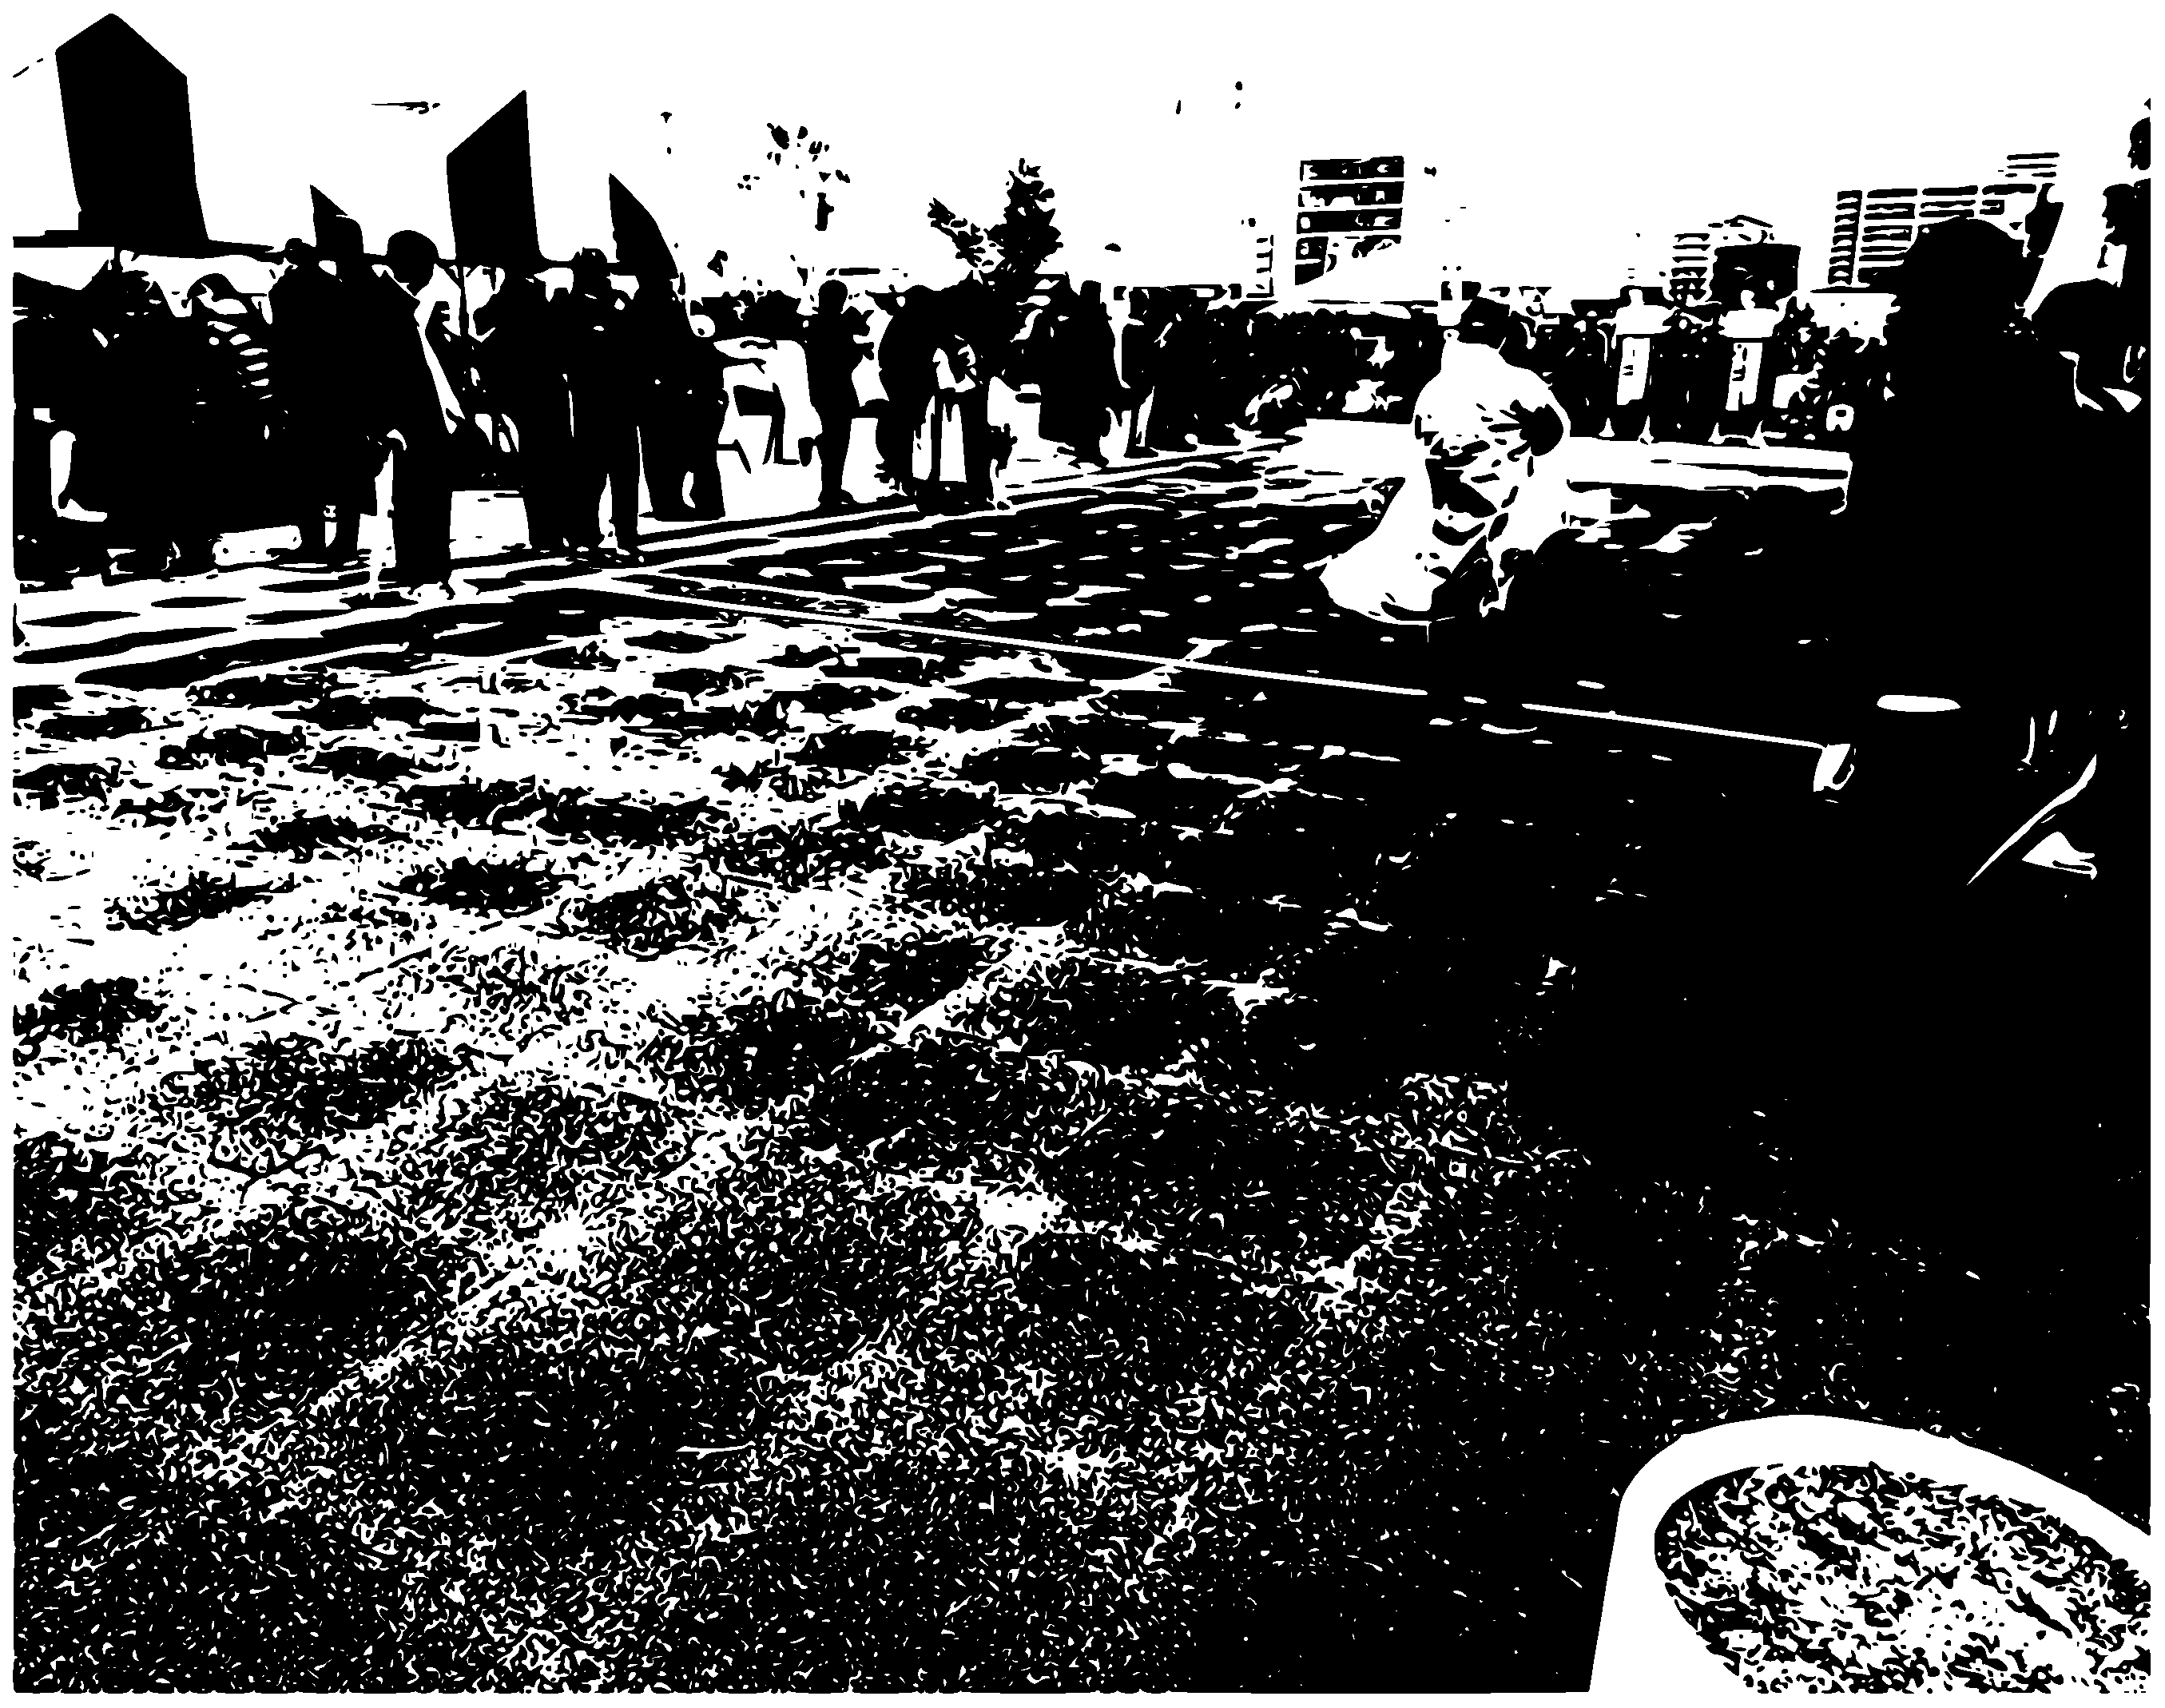
\includegraphics[height=38mm]{fig/hitogomi.eps}
   \vspace*{-4mm}
   \caption{Crowds at the start of the Tsukuba Challenge 2022}
   \label{fig: つくばチャレンジ人混み}
 \end{figure}

\section{手法}%===========================

 主なアルゴリズムの流れを図\ref{fig: つくばチャレンジ人混み}に示す。
初期化の部分で各パーティクルごとにランダムな観測範囲を付与する。
次に、動作モデルと観測モデルによる更新、リサンプリングを行うことで、
未知障害物が含まれていないような観測範囲をMCLのアルゴリズムによって求める。


\subsection{各パーティクルの初期化}

各パーティクルの初期化時に各パーティクルに対して、
ランダムな観測を与える。
ランダムな観測とは、360°のうちの、ある角度分を観測としたものである。

\subsection{動作モデル}

動作モデルは、MCLのアルゴリズム通りである。

\subsection{観測モデル}

観測モデルでは、各パーティクルの入力として、生の観測を受け取る。
観測を受け取り、各パーティクルはランダムな観測範囲を元に観測を間引く。
間引いた観測を元に尤度場から、そのパーティクルの尤度を求める。
尤度をかけ合わせたものをそのパーティクルの重みとする。

\subsection{リサンプリング}

リサンプリングでは、パーティクルの重みの正規化を行う。
また、1割程度の各パーティクルに対してランダムな観測範囲を再付与させる。
これは、各パーティクルがある観測範囲を選択し続ける問題を避けることが目的である。

\section{実験}%===========================

\subsection{実験環境}

実験環境について、図\ref{fig: つくばチャレンジ人混み}に示す。
実験は、図\ref{fig: つくばチャレンジ人混み}のつくばチャレンジでの人混みの環境を模した
図\ref{fig: つくばチャレンジ人混みシミュレータ}のシミュレータ環境で行う。
シミュレータにはGazebo、ナビゲーションのシステムにROS Noeticを使用する。
今回、実験に用いるロボットは差動二輪型のロボットである。

\begin{table}[hbtp]
  \caption{experimental environment}
  \label{table:data_type}
  \centering
  \begin{tabular}{lcr}
    \hline
    CPU & Core™ i9-12900K × 24 \\
    GPU & GeForce RTX 2060 \\
    Ubuntu & 20.04 \\
    ROS  & Noetic \\
    Gazebo  &  9.0 \\
    \hline
  \end{tabular}
\end{table}

\begin{figure}[h]
  \centering
   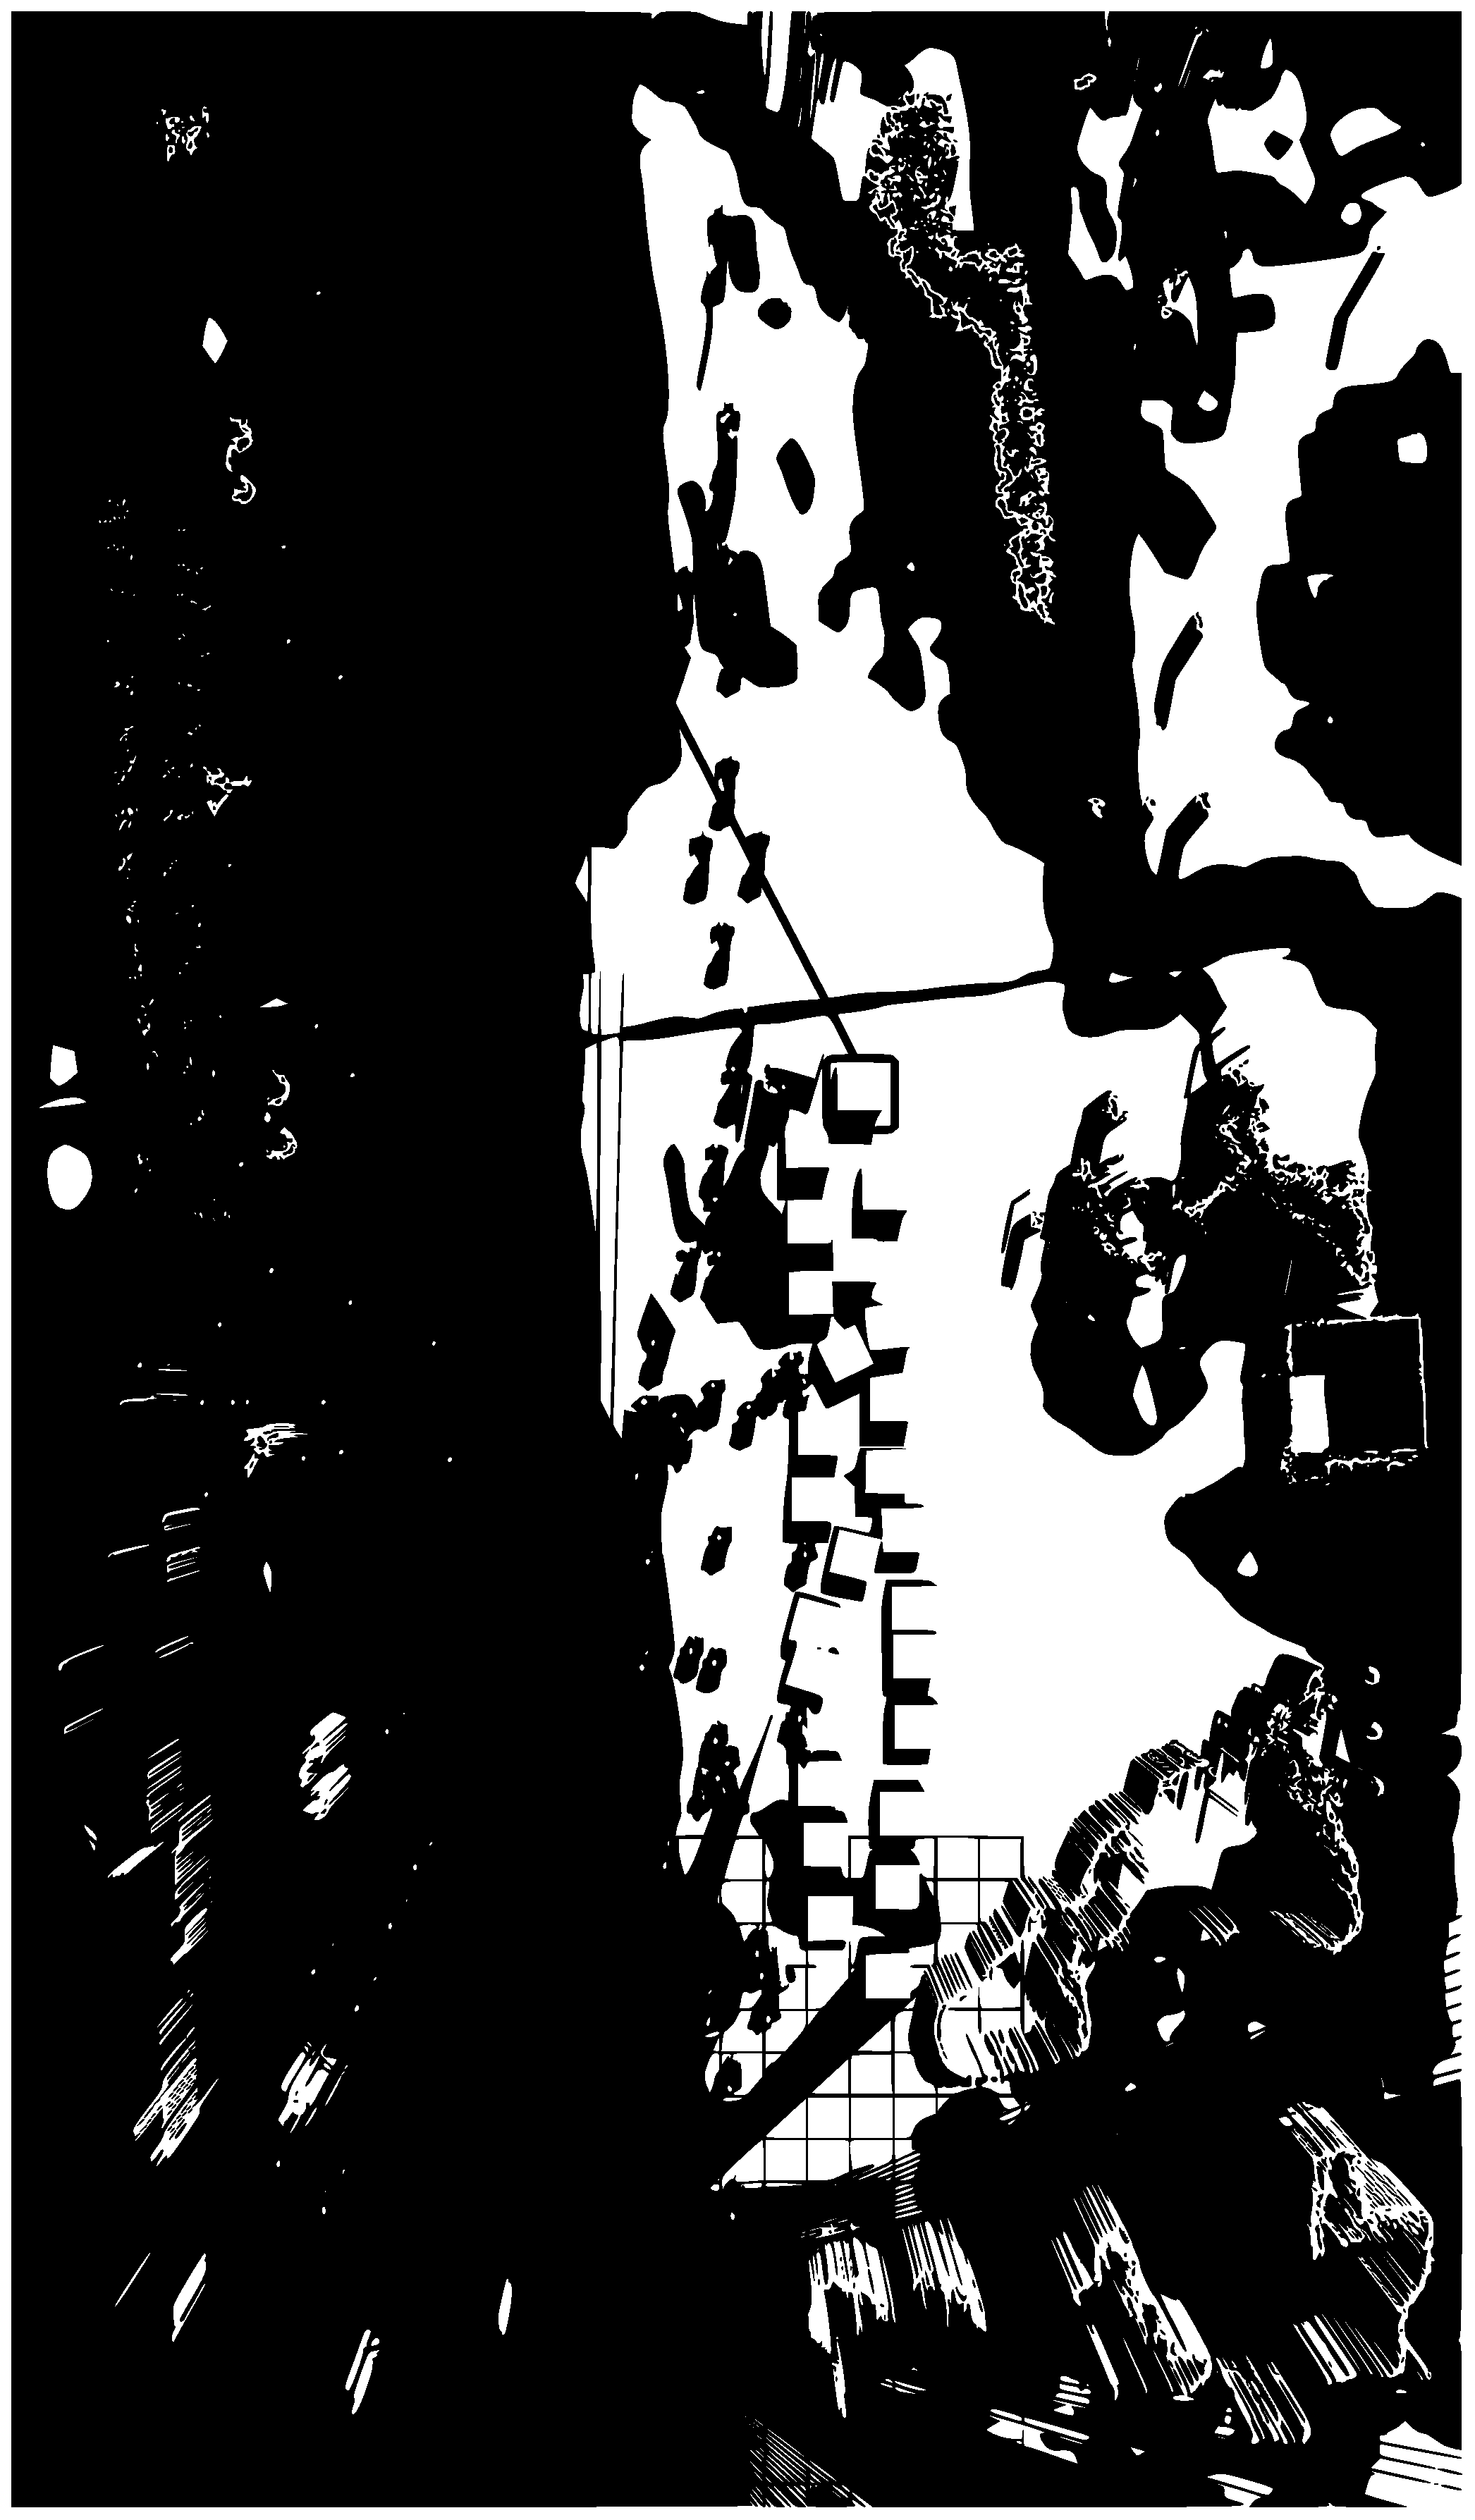
\includegraphics[height=140mm]{fig/simulator.eps}
   \vspace*{-4mm}
   \caption{A simulator that mimics the crowds at the start of Tsukuba Challenge 2022}
   \label{fig: つくばチャレンジ人混みシミュレータ}
 \end{figure}

\subsection{実験方法}

とする。

そのため、今回の実験での評価項目は以下のようになる。

\begin{itemize}
  \item スタートからゴールまでの完走率
  \begin{itemize}
    \item 未知障害物対応に最適な観測範囲
  \end{itemize}
  \item スタートからゴールまで走行したときの真値との比較
  \item 計算時間
\end{itemize}

\section{実験結果}%===========================

表\ref{table:data_type}に完走率の結果を示す。
試行量が足りているかということについては、
図\ref{fig: つくばチャレンジ人混み}を見ていただきたい。
各完走率の分布の重複部が少ないことから十分な試行であることがわかる。



\section{結言}%===========================


\footnotesize
\begin{thebibliography}{99}

\bibitem{MCL}

\bibitem{つくばチャレンジ}

\bibitem{富沢}

\bibitem{赤井}

\end{thebibliography}

\normalsize
\end{document}
